\documentclass[12pt,aspectratio=1610]{beamer}
\RequirePackage{
    amsmath,
    amssymb,
    calc,
    cancel,
    booktabs,
    color,
    siunitx,
    tikz,
    wrapfig,
    array,
    leftidx,
    float,
    etoolbox,
    fancyhdr,
    longtable,
    hyperref,
    ltcaption,
    ulem,
    wasysym,
    accents,
    listings,
    tabularx,
}

\hypersetup{
    hidelinks,
    breaklinks              = true,
}

\usepackage[final]{pdfpages}
\usepackage[many]{tcolorbox}

\RenewDocumentCommand{\vec}{m}{\mathbf{#1}}

\makeatletter
    \def\new@mathgroup{\alloc@8\mathgroup\mathchardef\@cclvi}
    \patchcmd{\document@select@group}{\sixt@@n}{\@cclvi}{}{}
    \patchcmd{\select@group}{\sixt@@n}{\@cclvi}{}{}
\makeatother

\RequirePackage{mathspec}                                   % includes fontspec
\RequirePackage{polyglossia}                                % multi-language support
\RequirePackage{xunicode}
\setdefaultlanguage{slovak}

% Setup fonts -- see fontspec/mathspec documentation.
\defaultfontfeatures{
    Mapping         = tex-text,
    Scale           = MatchLowercase,
    Ligatures       = TeX
}


\NewDocumentCommand{\labelmath}{m +m}{%
    \begin{equation}%
        #2%
        \label{#1}%
    \end{equation}%
}

\NewDocumentCommand{\labelalign}{m +m}{%
    \begin{align}%
        #2%
        \label{#1}%
    \end{align}%
}

\linespread{1.0}
\setlength{\parindent}{0cm}
\setlength{\parskip}{6pt}
\setlength{\abovedisplayskip}{0mm}
\setlength{\belowdisplayskip}{0mm}
\setlength{\abovedisplayshortskip}{0mm}
\setlength{\belowdisplayshortskip}{0mm}
\setlength{\itemindent}{0pt}
\setlength{\textfloatsep}{0mm}
\setlength{\tabcolsep}{3mm}
\setlength{\LTcapwidth}{0.8\textwidth}
\renewcommand{\arraystretch}{1.2}

\setcounter{secnumdepth}{2}

/home/kvik/dgs/core/tex/math.tex
\DeclareSIUnit\au{AU}
\DeclareSIUnit\pixel{px}
\DeclareSIUnit\lightyear{ly}
\DeclareSIUnit\parsec{pc}
\DeclareSIUnit\earthmass{M_{\earth}}
\DeclareSIUnit\speedoflight{c}
\DeclareSIUnit\foe{foe}
\DeclareSIUnit\year{yr}
\DeclareSIUnit\eur{€}
\DeclareSIUnit\solarmass{M_{\astrosun}}
\DeclareSIUnit\solarluminosity{L_{\astrosun}}
\DeclareSIUnit{\byte}{B}




\linespread{1.0}
\setlength{\parindent}{0cm}
\setlength{\parskip}{6pt}
\setlength{\abovedisplayskip}{0mm}
\setlength{\belowdisplayskip}{0mm}
\setlength{\abovedisplayshortskip}{0mm}
\setlength{\belowdisplayshortskip}{0mm}
\setlength{\itemindent}{0pt}
\setlength{\textfloatsep}{0mm}
\setlength{\tabcolsep}{3mm}
\renewcommand{\arraystretch}{1.2}

\setcounter{secnumdepth}{0}

\NewDocumentCommand{\fspicture}{m O{W} O{black}}{
    {
        \setbeamertemplate{navigation symbols}{}
        \setbeamercolor{background canvas}{bg = #3}
        \begin{frame}[plain]
            \begin{tikzpicture}[remember picture, overlay]
                \node[at=(current page.center)] {
                    \ifstrequal{H}{#2}{                                  
                        \includegraphics[height=\paperheight]{#1}%
                    }{%
                        \includegraphics[width=\paperwidth]{#1}%
                    }
                };
            \end{tikzpicture}
        \end{frame}
    }
}

\NewDocumentCommand{\frejm}{m +m}{
    \begin{frame}
        \frametitle{#1}
        #2
    \end{frame}
}

\NewDocumentCommand{\fragfrejm}{m +m}{
    \begin{frame}[fragile]
        \frametitle{#1}
        #2
    \end{frame}
}

\defbeamertemplate{description item}{align center}{\hfill\insertdescriptionitem\hfill}
\definecolor{desc}{rgb}{0.66, 0, 0}
\definecolor{citem}{rgb}{0.72, 0, 0}
\definecolor{csitem}{rgb}{0.90, 0, 0}
\definecolor{cssitem}{rgb}{1, 0.1, 0.1}
\definecolor{qprimarybg}{rgb}{0.95, 0.95, 0.95}
\definecolor{check}{rgb}{0, 0.8, 0}
\definecolor{coded}{rgb}{0.9, 0.9, 0.9}
\definecolor{todo}{rgb}{1.0, 0.3, 0.3}
\definecolor{model}{rgb}{0.75, 0, 0}

\setbeamertemplate{navigation symbols}{}
\newfontfamily{\semibold}{Segoe UI Semibold}
\RenewDocumentCommand{\emph}{m}{{\semibold#1}}
\NewDocumentCommand{\code}{m}{\textcolor{desc}{\texttt{#1}}}
\NewDocumentCommand{\model}{m}{\colorbox{coded}{\textcolor{model}{\texttt{#1}}}}
\NewDocumentCommand{\todo}{m}{\colorbox{todo}{#1}}

\mode<presentation> {
    \usetheme{Szeged}
    \usecolortheme{beaver}
    
    \usefonttheme{professionalfonts}
    \setallmainfonts{Minion Pro}
    \setmathrm{Minion Pro}
    
    \setsansfont{Segoe UI}
    \setmonofont{Consolas}
    \setbeamercolor*{enumerate item}{fg = citem}
    \setbeamercolor*{enumerate subitem}{fg = csitem}
    \setbeamercolor*{enumerate subsubitem}{fg = cssitem}
    \setbeamercolor*{description item}{fg = desc}
    \setbeamercolor*{itemize item}{fg = citem}
    \setbeamercolor*{itemize subitem}{fg = csitem}
    \setbeamercolor*{itemize subsubitem}{fg = cssitem}
    \setbeamercolor*{palette primary}{fg = red, bg = qprimarybg}
}

\newcommand<>\highlightbox[2]{%
    \alt#3{\makebox[\dimexpr\width-2\fboxsep]{\colorbox{#1}{#2}}}{#2}%
}

\AtBeginSection[]{
    \subsection{\insertsection}
    \begin{frame}
        \vfill
        \centering
        \begin{beamercolorbox}[sep = 18pt, center, shadow = true, rounded = true]{title}
            \usebeamerfont{title}\insertsectionhead%
            \vfill
        \end{beamercolorbox}
        \vfill
    \end{frame}
}

\makeatletter
% Render percent sign with nice font, not ugly Computer modern
    \mathcode`\%="7025

% Fixes mathspec bug -- URL numbers are rendered with wrong font
    \ernewcommand\eu@MathPunctuation@symfont{Latin:m:n}
    \DeclareMathSymbol{,}{\mathpunct}{\eu@MathPunctuation@symfont}{`,}
    \DeclareMathSymbol{?}{\mathpunct}{\eu@MathPunctuation@symfont}{`?}
    \DeclareMathSymbol{.}{\mathord}{\eu@MathPunctuation@symfont}{`.}
    \DeclareMathSymbol{<}{\mathrel}{\eu@MathPunctuation@symfont}{`<}
    \DeclareMathSymbol{>}{\mathrel}{\eu@MathPunctuation@symfont}{`>}
    \DeclareMathSymbol{/}{\mathord}{\eu@MathPunctuation@symfont}{`/}
    \DeclareMathSymbol{;}{\mathpunct}{\eu@MathPunctuation@symfont}{`;}
    \DeclareMathSymbol{(}{\mathopen}{\eu@DigitsArabic@symfont}{`(}
    \DeclareMathSymbol{)}{\mathclose}{\eu@DigitsArabic@symfont}{`)}
    \XeTeXDeclareMathSymbol{^^^^2026}{\mathinner}{\eu@MathPunctuation@symfont}{"2026}[\mathellipsis]
    \DeclareMathSymbol{0}{\mathalpha}{\eu@DigitsArabic@symfont}{`0}
    \DeclareMathSymbol{1}{\mathalpha}{\eu@DigitsArabic@symfont}{`1}
    \DeclareMathSymbol{2}{\mathalpha}{\eu@DigitsArabic@symfont}{`2}
    \DeclareMathSymbol{3}{\mathalpha}{\eu@DigitsArabic@symfont}{`3}
    \DeclareMathSymbol{4}{\mathalpha}{\eu@DigitsArabic@symfont}{`4}
    \DeclareMathSymbol{5}{\mathalpha}{\eu@DigitsArabic@symfont}{`5}
    \DeclareMathSymbol{6}{\mathalpha}{\eu@DigitsArabic@symfont}{`6}
    \DeclareMathSymbol{7}{\mathalpha}{\eu@DigitsArabic@symfont}{`7}
    \DeclareMathSymbol{8}{\mathalpha}{\eu@DigitsArabic@symfont}{`8}
    \DeclareMathSymbol{9}{\mathalpha}{\eu@DigitsArabic@symfont}{`9}
\makeatother


\title{Investigation of meteor models with numerical simulation}
\subtitle{Toying with models of meteor flight for a deeper understanding}
\author{\small \emph{Martin Baláž} \\ Juraj Tóth, PhD. \\ Peter Vereš, PhD.}
\institute{IMC 2019, Bollmannsruh}
\date{2019--10--05}

\begin{document}
    {
        \usebackgroundtemplate{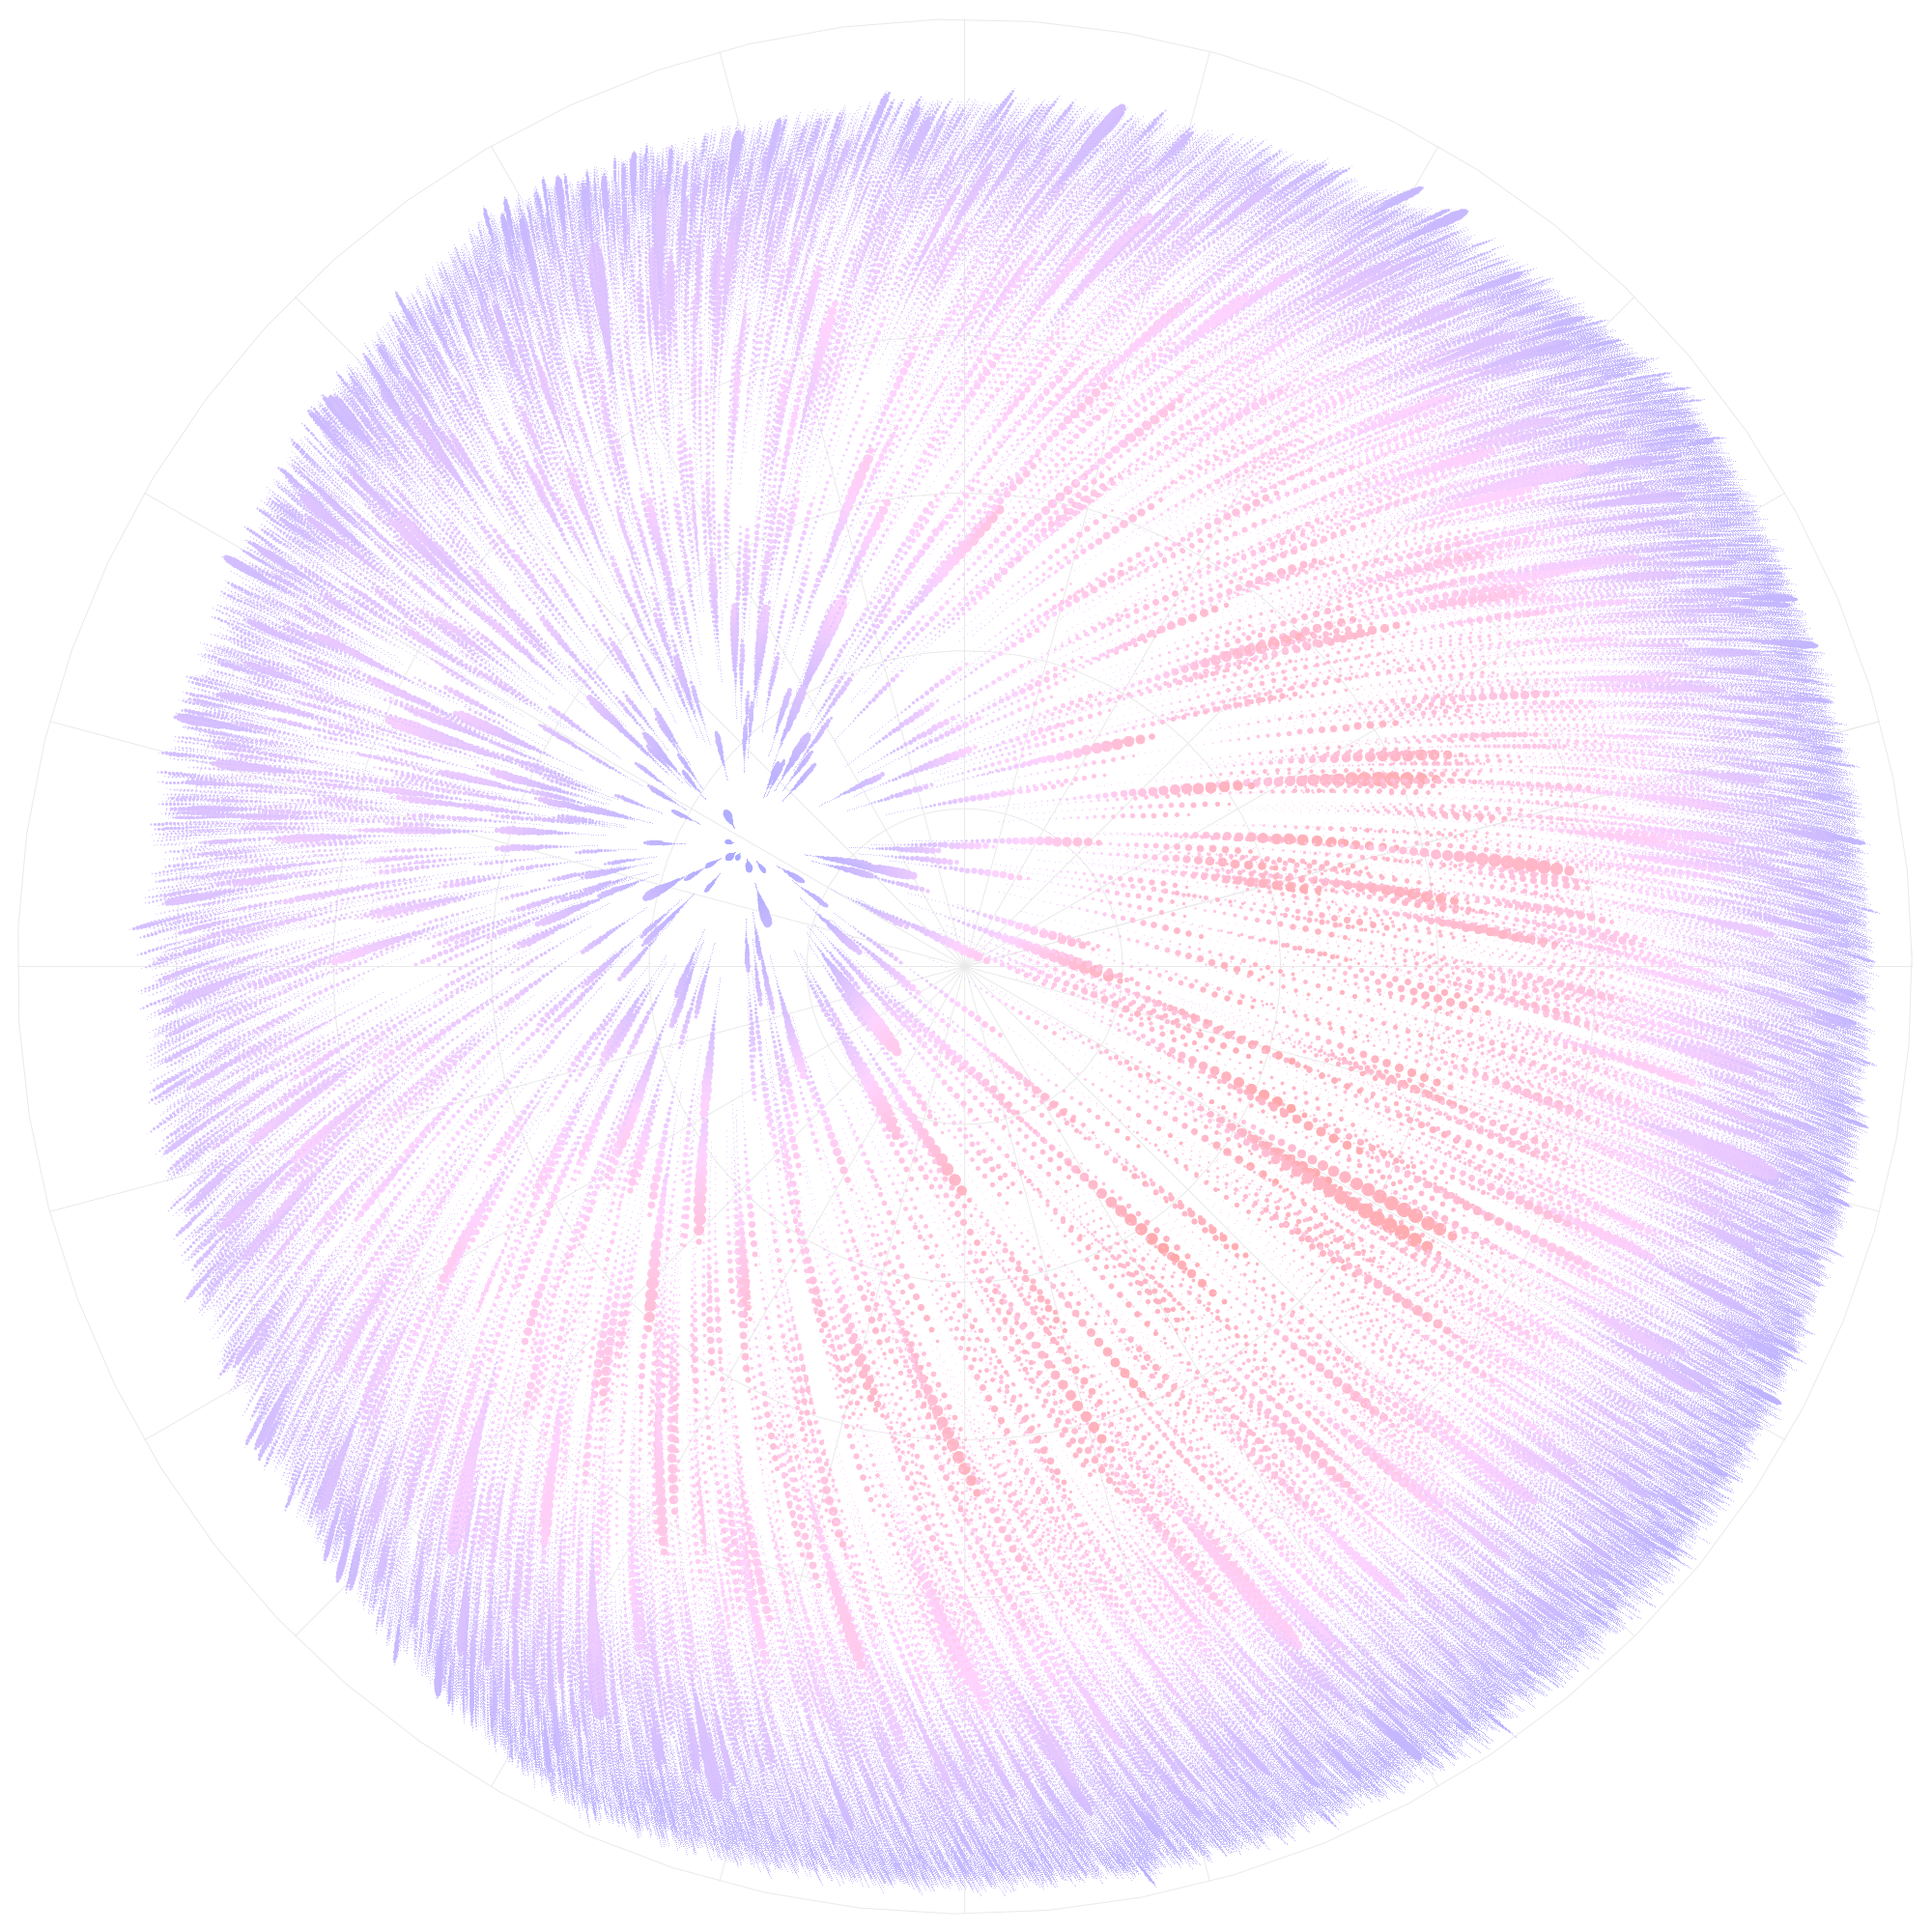
\includegraphics[width=\paperwidth]{fireworks-i.png}}
        \begin{frame}
            \titlepage
        \end{frame}
    }
                
    \section{Overview}
        \frejm{What am I developing}{
            \begin{itemize}
                \item a (more-or-less) universal meteor simulator
                \pause
                \item we can
                \begin{itemize}
                    \item estimate meteor flux
                    \item validate physical models
                    \item fit observations
                    \item ...
                \end{itemize}
                \pause
                \item work in progress
            \end{itemize}
            \begin{itemize}
                \item let's take it beyond statistics
            \end{itemize}

        }

        \frejm{Algorithm}{
            \begin{enumerate}
                \item generate the meteoroid population
                \pause
                \item simulate atmospheric entry
                \pause
                \item compute meteor sightings
                    \begin{itemize}
                        \item position in the sky
                        \item magnitude
                        \item entry angle
                        \item ...
                    \end{itemize}
                \pause
                \item look at the dataset
            \end{enumerate}
        }
						
    \setbeamersize{description width = 5mm}
    \section{Simulation}
        % This time we are investigating the models
        %\frejm{Model}{            
        %    \emph{Whipple} (1938), improved by \emph{Öpik} (1955) and \emph{Ceplecha} (2001)
        %    
        %    We assume
        %    \begin{itemize}
        %        \item spherical, continuously ablating particles
        %    \end{itemize}
        %    
        %    We need
        %    \begin{itemize}
        %        \item equations of motion
        %        \item equation of luminance
        %        \item atmospheric and instrumental effects
        %        \item to compute the statistic
        %    \end{itemize}            
        %}
    
        %\frejm{Equations of motion}{
        %    \begin{itemize}
        %        \item braking equation
        %        $$
        %            \diff{v} = -\frac{\Gamma A}{m^{1/3} \rho^{2/3}} \rho_{\mathrm{air}} v^2 \diff{t}
        %        $$
        %        \item equation of ablation
        %        $$
        %            \diff{m} = -\frac{\Lambda A}{2Q} \frac{m^{2/3}}{\rho^{2/3}} \rho_{\mathrm{air}} v^3 \diff{t}
        %        $$
        %        \item equation of luminance
        %        $$
        %            L = \tau(v) \frac{\Lambda A}{4Q} \frac{m^{2/3}}{\rho^{2/3}} \rho_{\mathrm{air}} v^5
        %        $$
        %        \begin{itemize}
        %            \item $\tau(v)$ determined by \emph{Jones \& Halliday (2001)}
        %        \end{itemize}
        %    \end{itemize}
        %}
        
        \frejm{Simulation of flight}{
            \emph{Runge--Kutta} integrator (RK4)
            \begin{itemize}
                \item complete ablation of the particle
                \pause
                \item \emph{snapshots} taken $N$ times per second
                \pause
                \item multiple integration steps
            \end{itemize}
        }
        
        \fspicture{angularSpeed-teplicne-streaks.png}[H][black]
                 
        \fspicture{mjd-entryAngle-appMag.png}
        \fspicture{logInitMass-absMag-appMag.png}
        \fspicture{absMag-elevation-appMag.png}

    \section{Prerequisites}
        \frejm{Random generator}{
            \begin{itemize}
                \item  approximate the real population
                \begin{itemize}
                    \item easy for \emph{showers}
                    \item \emph{very difficult} for sporadic background
                \end{itemize}
                \pause
                \item $\pm$ constant $\vec{v}$
                \item slowly varying activity
            \end{itemize}
        }

        \frejm{Grid generator}{
            Plain old scientific method...
            \pause
            \begin{itemize}
                \item fix all parameters of meteoroids...
                \pause
                \item ...except one...
                \pause
                \item ...vary it slowly
            \end{itemize}
            \pause
            \begin{itemize}
                \item simulate, observe, analyze...
                \item look for changes in the output
            \end{itemize}
            
            \pause
            We may analyze either \emph{max-light frame} or \emph{entire trail}
        }
        %picture maxlight vs trail

        \fspicture{grid-sky.png}[H]

        \frejm{Constraints}{
            We simplify things (unless stated otherwise)
            \begin{itemize}                
                \item observer at North pole
                \item constant atmospheric model
                \item start in zenith
            \end{itemize}
            \pause
            \begin{itemize}                
                \item scatter plot
                \item colour by varied property
                \item emphasize max-light frame
            \end{itemize}
        }

    \section{Entry angle}
        \frejm{Parameters}{
            varying \emph{declination} = \emph{entry angle}
            \begin{itemize}
                \item mass \SI{1}{\gram}
            \end{itemize}
        }

        \fspicture{ea-tme.png}
        \fspicture{ea-the.png}
        \fspicture{ea-Mae.png}
        \fspicture{ea-tLe.png}

    \section{Mass}
        \frejm{Parameters}{
            \begin{itemize}
                \item Perseids
                \begin{itemize}
                    \item material, radiant, velocity, ...
                \end{itemize}
                \pause
                \item mass from \SI{1e-6}{\kilo\gram} to \SI{1}{\kilo\gram}
                \item logarithmic spacing
            \end{itemize}
        }
        %pictures

        \frejm{Results}{
            \begin{itemize}
                \item maximum brightness at ~1/3 initial mass
                \item VERIFY THIS FOR MULTIPLE VARIATIONS
            \end{itemize}
        }
        
    \section{Heat of ablation}
        \frejm{Parameters}{
            \begin{itemize}
                \item $Q$ \SIrange{1e3}{1e9}{\joule\per\kilo\gram}
                \item 
                \item wildly non-linear behaviour
            \end{itemize}
        }
        %\fspicture{hoa-.png}

        \frejm{Density}{
            \begin{itemize}

            \end{itemize}
        }

        \frejm{Speed}{
            revise \emph{High geocentric velocity meteor ablation} (Hill et al., 2005)
        }

    \section{Conclusion}
        \frejm{Validation}{
            Revise other simulations (Gural)
        }

        \frejm{Deficiencies of the model}{
            \begin{itemize}
                \item not dependent on $\Gamma$
            \end{itemize}
        }

        \frejm{Ultimate goal}{
            \begin{itemize}
                \item revise the physics 
                \item hopefully design a better one
                \begin{itemize}
                    \item compare with real meteors
                    \item use in flux estimations
                \end{itemize}
            \end{itemize}
        }

        \frejm{Summary}{
            \begin{itemize}
                \item versatile, universal tool
                \item applicable to \emph{almost any} meteor observing system
            \end{itemize}
            \pause
            \begin{itemize}
                \item the tools are \emph{open-source}
                \begin{itemize}
                    \item \url{https://github.com/sesquideus/asmodeus}
                \end{itemize}
                \item suggestions or comments welcome
            \end{itemize}
        }
        
        \frejm{References}{
            \begin{itemize}
                \item \textbf{Öpik, E. J.}:
                    Physics of meteor flight in the atmosphere. Interscience Publishers, 1958.  
                \item \textbf{Hill, K. A. -- Rogers, L. A. -- Hawkes, R. L.}:
                    High geocentric velocity meteor ablation. Astronomy \& Astrophysics 444, 615--624 (2005) 
                \item \textbf{Jones, W. -- Halliday, I.}:
                    Effects of Excitation and Ionization in Meteor Trains. MNRAS vol. 321, 2001, pp417--423.
            \end{itemize}
        }
            
\end{document}
